\documentclass[10pt,aspectratio=169]{beamer}

%% package to add notes to slides 
%\usepackage{pgfpages}
%\setbeameroption{show notes}
%\setbeameroption{show notes on second screen=right}

\usepackage{hyperref}
\usepackage{xcolor}
\usepackage{pythonhighlight}
\usepackage{FiraSans}

% Graphics preamble
\usepackage{graphicx} % import graphics package
%\graphicspath{ {/Users/tgol0003/Desktop/seagate4_2/uwgeo_models/production_models/} } % harddisk path
\usepackage{float} % Allows for control of float positions
\usepackage[section]{placeins} % to place figures in the section 
\usepackage{multicol} % position figures across the columns

\usetheme{metropolis}
\usepackage{appendixnumberbeamer}

\usepackage{booktabs}
\usepackage[scale=2]{ccicons}

\usepackage{pgfplots}
\usepgfplotslibrary{dateplot}

\usepackage{xspace}
\newcommand{\themename}{\textbf{\textsc{metropolis}}\xspace}

\title{Annulus Benchmarks}
\subtitle{Underworld3}
\date{\today}
\author{Thyagarajulu Gollapalli \& Underworld Team}
\institute{Monash University}
% \titlegraphic{\hfill\includegraphics[height=1.5cm]{logo.pdf}}

\begin{document}

\maketitle

\begin{frame}{Table of contents}
  \setbeamertemplate{section in toc}[sections numbered]
  \tableofcontents[hideallsubsections]
%  \note[item]{Welcome to the talk!} adding notes
\end{frame}

\section{Introduction}

\begin{frame}[fragile]{What are Annulus Benchmarks?}
	Fill information here later...
\end{frame}

\begin{frame}[fragile]{What is Underworld3?}
	Fill information here later...
\end{frame}

\begin{frame}[fragile]{What is Underworld3?}
	Fill information here later...
\end{frame}

\begin{frame}[fragile]{Solving for...}
	Incompressible Stokes flow in an annulus:
	\begin{itemize}
		\item Constant viscosity
		\item Gravity field that points towards the center of an annulus
		\item Density field that depends on the spatial coordinates
	\end{itemize}
\end{frame}

\begin{frame}[fragile]{Which FEM cells are used? Why?}
	Fill information here later...
\end{frame}

\begin{frame}[fragile]{What is Penalty Method?}
	Fill information here later...
\end{frame}

\section{Annulus Benchmark: Thieulot}

\begin{frame}{Analytical Equations}
	This benchmark is based on a manufactured solution in which an analytical solution to the isoviscous incompressible Stokes equations is derived in an annulus geometry. The velocity and pressure fields are as follows:
	
	$$ v_{\theta}(r, \theta) = f(r) \cos(k\theta) $$
	$$ v_r(r, \theta) = g(r)k \sin(k\theta) $$
	$$ p(r, \theta) = kh(r) \sin(k\theta) + \rho_0g_r(R_2 - r) $$
	$$ \rho(r, \theta) = m(r)k \sin(k\theta) + \rho_0 $$
	
	with
	$$ f(r) = Ar + \frac{B}{r} $$
	$$ g(r) = \frac{A}{2}r + \frac{B}{r}\ln r + \frac{C}{r} $$
	
\end{frame}

\begin{frame}{Analytical Equations (Continued)}
	
	$$ h(r) = \frac{2g(r) - f(r)}{r} $$
	$$ m(r) = g''(r) - \frac{g'(r)}{r} - \frac{g(r)}{r^2}(k^2 - 1) + \frac{f(r)}{r^2} + \frac{f'(r)}{r} $$
	$$ A = -C\frac{2(\ln R_1 - \ln R_2)}{R_2^2 \ln R_1 - R_1^2 \ln R_2} $$
	$$ B = -C\frac{R_2^2 - R_1^2}{R_2^2 \ln R_1 - R_1^2 \ln R_2} $$
	
	The parameters $A$ and $B$ are chosen so that $ v_r(R_1, \theta) = v_r(R_2, \theta) = 0 $ for all $\theta \in [0, 2\pi]$, i.e. the velocity is tangential to both inner and outer surfaces. The gravity vector is radial inward and of unit length.
	
	The parameter $k$ controls the number of convection cells present in the domain.
	
	In the present case, we set $ R_1 = 1, R_2 = 2$ and $C = -1 $.
\end{frame}

\begin{frame}[fragile]{Boundary Condition}
	\begin{python}
		# boundary condition
		v_diff =  v_uw.sym - v_ana.sym
		stokes.add_natural_bc(vel_penalty*v_diff, "Upper")
		stokes.add_natural_bc(vel_penalty*v_diff, "Lower")
	\end{python}
\end{frame}

%\begin{frame}[fragile]{Mesh}
%	\begin{figure}[!htb]
%		\begin{multicols}{4}
%			\includegraphics[width=3.5cm]{../output/Latex_Dir/model_k_0_res_32_vdeg_2_pdeg_1_pcont_True_vel_penalty_1.0e+08_stokes_tol_1.0e-10/mesh.png}\par
%			\hspace{0.75in}
%			\includegraphics[width=3.5cm]{../output/Latex_Dir/model_k_1_res_32_vdeg_2_pdeg_1_pcont_True_vel_penalty_1.0e+08_stokes_tol_1.0e-10/mesh.png}\par
%			\hspace{1.5in}
%			\includegraphics[width=3.5cm]{../output/Latex_Dir/model_k_2_res_32_vdeg_2_pdeg_1_pcont_True_vel_penalty_1.0e+08_stokes_tol_1.0e-10/mesh.png}\par
%			\hspace{2.25in}
%			\includegraphics[width=3.5cm]{../output/Latex_Dir/model_k_4_res_32_vdeg_2_pdeg_1_pcont_True_vel_penalty_1.0e+08_stokes_tol_1.0e-10/mesh.png}
%		\end{multicols}
%	\end{figure}
%\end{frame}

\begin{frame}[fragile]{Density Distribution}
	\begin{figure}[!htb]
		\begin{multicols}{4}
			\includegraphics[width=3.5cm]{../output/Latex_Dir/model_k_0_res_32_vdeg_2_pdeg_1_pcont_True_vel_penalty_1.0e+08_stokes_tol_1.0e-10/rho_ana.png}\par
			\hspace{0.75in}
			\includegraphics[width=3.5cm]{../output/Latex_Dir/model_k_1_res_32_vdeg_2_pdeg_1_pcont_True_vel_penalty_1.0e+08_stokes_tol_1.0e-10/rho_ana.png}\par
			\hspace{1.5in}
			\includegraphics[width=3.5cm]{../output/Latex_Dir/model_k_2_res_32_vdeg_2_pdeg_1_pcont_True_vel_penalty_1.0e+08_stokes_tol_1.0e-10/rho_ana.png}\par
			\hspace{2.25in}
			\includegraphics[width=3.5cm]{../output/Latex_Dir/model_k_4_res_32_vdeg_2_pdeg_1_pcont_True_vel_penalty_1.0e+08_stokes_tol_1.0e-10/rho_ana.png}\par
		\end{multicols}
	\end{figure}
	
	\vspace{-0.4in}
	
	\begin{figure}
		\hspace{0.2in} 
		\includegraphics[width=5cm]{../output/Latex_Dir/model_k_0_res_32_vdeg_2_pdeg_1_pcont_True_vel_penalty_1.0e+08_stokes_tol_1.0e-10/rho_ana_cbhorz.pdf}
	\end{figure}
\end{frame}

\begin{frame}{Analytical Solution}
	\vspace{-0.32in}
	\begin{figure}[!htb]
		\begin{multicols}{4}
			\includegraphics[width=3.5cm]{../output/Latex_Dir/model_k_0_res_32_vdeg_2_pdeg_1_pcont_True_vel_penalty_1.0e+08_stokes_tol_1.0e-10/vel_ana.png}\par
			\hspace{0.75in}
			\includegraphics[width=3.5cm]{../output/Latex_Dir/model_k_1_res_32_vdeg_2_pdeg_1_pcont_True_vel_penalty_1.0e+08_stokes_tol_1.0e-10/vel_ana.png}\par
			\hspace{1.5in}
			\includegraphics[width=3.5cm]{../output/Latex_Dir/model_k_2_res_32_vdeg_2_pdeg_1_pcont_True_vel_penalty_1.0e+08_stokes_tol_1.0e-10/vel_ana.png}\par
			\hspace{2.25in}
			\includegraphics[width=3.5cm]{../output/Latex_Dir/model_k_4_res_32_vdeg_2_pdeg_1_pcont_True_vel_penalty_1.0e+08_stokes_tol_1.0e-10/vel_ana.png}
		\end{multicols}
		\vspace{-0.29in}
		\begin{figure}
			\hspace{0.1in} 
			\includegraphics[width=3cm]{../output/Latex_Dir/model_k_0_res_32_vdeg_2_pdeg_1_pcont_True_vel_penalty_1.0e+08_stokes_tol_1.0e-10/v_ana_cbhorz.pdf}
		\end{figure}
	\end{figure}
	
	\begin{figure}[!htb]
		\vspace{-0.5in}
		\begin{multicols}{4}
			\includegraphics[width=3.5cm]{../output/Latex_Dir/model_k_0_res_32_vdeg_2_pdeg_1_pcont_True_vel_penalty_1.0e+08_stokes_tol_1.0e-10/p_ana.png}\par
			\hspace{0.75in}
			\includegraphics[width=3.5cm]{../output/Latex_Dir/model_k_1_res_32_vdeg_2_pdeg_1_pcont_True_vel_penalty_1.0e+08_stokes_tol_1.0e-10/p_ana.png}\par
			\hspace{1.5in}
			\includegraphics[width=3.5cm]{../output/Latex_Dir/model_k_2_res_32_vdeg_2_pdeg_1_pcont_True_vel_penalty_1.0e+08_stokes_tol_1.0e-10/p_ana.png}\par
			\hspace{2.25in}
			\includegraphics[width=3.5cm]{../output/Latex_Dir/model_k_4_res_32_vdeg_2_pdeg_1_pcont_True_vel_penalty_1.0e+08_stokes_tol_1.0e-10/p_ana.png}
		\end{multicols}
		\vspace{-0.27in}
		\begin{figure}
			\hspace{0.1in} 
			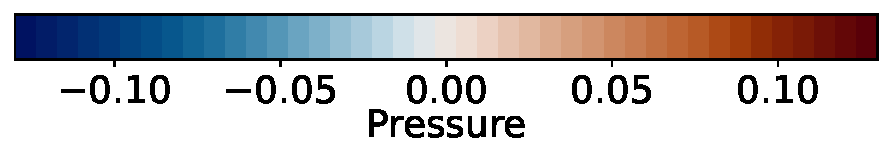
\includegraphics[width=3cm]{../output/Latex_Dir/model_k_0_res_32_vdeg_2_pdeg_1_pcont_True_vel_penalty_1.0e+08_stokes_tol_1.0e-10/p_ana_cbhorz.pdf}
		\end{figure}
	\end{figure}
\end{frame}

\begin{frame}{Numerical Solution}
	\vspace{-0.32in}
	\begin{figure}[!htb]
		\begin{multicols}{4}
			\includegraphics[width=3.5cm]{../output/Latex_Dir/model_k_0_res_32_vdeg_2_pdeg_1_pcont_True_vel_penalty_1.0e+08_stokes_tol_1.0e-10/vel_uw.png}\par
			\hspace{0.75in}
			\includegraphics[width=3.5cm]{../output/Latex_Dir/model_k_1_res_32_vdeg_2_pdeg_1_pcont_True_vel_penalty_1.0e+08_stokes_tol_1.0e-10/vel_uw.png}\par
			\hspace{1.5in}
			\includegraphics[width=3.5cm]{../output/Latex_Dir/model_k_2_res_32_vdeg_2_pdeg_1_pcont_True_vel_penalty_1.0e+08_stokes_tol_1.0e-10/vel_uw.png}\par
			\hspace{2.25in}
			\includegraphics[width=3.5cm]{../output/Latex_Dir/model_k_4_res_32_vdeg_2_pdeg_1_pcont_True_vel_penalty_1.0e+08_stokes_tol_1.0e-10/vel_uw.png}
		\end{multicols}
		\vspace{-0.29in}
		\begin{figure}
			\hspace{0.1in} 
			\includegraphics[width=3cm]{../output/Latex_Dir/model_k_0_res_32_vdeg_2_pdeg_1_pcont_True_vel_penalty_1.0e+08_stokes_tol_1.0e-10/v_ana_cbhorz.pdf}
		\end{figure}
	\end{figure}
	
	\begin{figure}[!htb]
		\vspace{-0.5in}
		\begin{multicols}{4}
			\includegraphics[width=3.5cm]{../output/Latex_Dir/model_k_0_res_32_vdeg_2_pdeg_1_pcont_True_vel_penalty_1.0e+08_stokes_tol_1.0e-10/p_uw.png}\par
			\hspace{0.75in}
			\includegraphics[width=3.5cm]{../output/Latex_Dir/model_k_1_res_32_vdeg_2_pdeg_1_pcont_True_vel_penalty_1.0e+08_stokes_tol_1.0e-10/p_uw.png}\par
			\hspace{1.5in}
			\includegraphics[width=3.5cm]{../output/Latex_Dir/model_k_2_res_32_vdeg_2_pdeg_1_pcont_True_vel_penalty_1.0e+08_stokes_tol_1.0e-10/p_uw.png}\par
			\hspace{2.25in}
			\includegraphics[width=3.5cm]{../output/Latex_Dir/model_k_4_res_32_vdeg_2_pdeg_1_pcont_True_vel_penalty_1.0e+08_stokes_tol_1.0e-10/p_uw.png}
		\end{multicols}
		\vspace{-0.27in}
		\begin{figure}
			\hspace{0.1in} 
			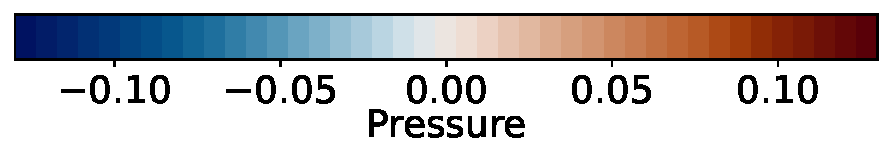
\includegraphics[width=3cm]{../output/Latex_Dir/model_k_0_res_32_vdeg_2_pdeg_1_pcont_True_vel_penalty_1.0e+08_stokes_tol_1.0e-10/p_ana_cbhorz.pdf}
		\end{figure}
	\end{figure}
\end{frame}

\begin{frame}{Error Convergence}
	Velocity penalty: 2.5e6 (magenta), 1e8 (green), 1e10 (skyblue) \newline
	Stokes tolerance: 1e-10 \newline
	Stokes element: $P_{2}P_{1}$
	\begin{figure}[!htb]
		\begin{multicols}{2}
			\includegraphics[width=7cm]{../output/Annulus_Benchmark_Thieulot/benchmark_figs/vel_err_conv_vel_penalty_1.0e+10_stokes_tol_1.0e-10_all_v_pen.pdf}\par
			\hspace{3.0in} 
			\includegraphics[width=7cm]{../output/Annulus_Benchmark_Thieulot/benchmark_figs/p_err_conv_vel_penalty_1.0e+10_stokes_tol_1.0e-10_all_v_pen.pdf}
		\end{multicols}
	\end{figure}
\end{frame}

\begin{frame}{Error Convergence}
	Stokes elements: $P_{1}P_{0} (disc. pressure), P_{2}P_{1}, P_{3}P_{2}$  \newline
	Velocity penalty: 2.5e6, 1e10, 1e10 \newline
	Stokes tolerance: 1e-7, 1e-10, 1e-10
	\begin{figure}[!htb]
		\begin{multicols}{2}
			\includegraphics[width=7cm]{../output/Annulus_Benchmark_Thieulot/benchmark_figs/vel_err_conv_vel_penalty_1.0e+10_stokes_tol_1.0e-10_all_k.pdf}\par
			\hspace{3.0in} 
			 \includegraphics[width=7cm]{../output/Annulus_Benchmark_Thieulot/benchmark_figs/p_err_conv_vel_penalty_1.0e+10_stokes_tol_1.0e-10_all_k.pdf}
		\end{multicols}
	\end{figure}
\end{frame}

\begin{frame}{Conclusions}

\end{frame}

\section{Annulus Benchmark: Kramer}

\begin{frame}{Analytical Equations}
	Detailed derivation of the analytical equations are found:
	
	\href{https://gmd.copernicus.org/articles/14/1899/2021/}{\textcolor{magenta}{Analytical solutions for mantle flow in cylindrical and spherical shells}}
	
	\vspace{0.25in}
	
	Python package to compute analytical solutions:
	
	\href{https://assess.readthedocs.io/en/latest/}{\textcolor{teal}{Assess}}
\end{frame}

\begin{frame}[fragile]{Boundary Condition}
	\begin{python}
		# boundary condition
		v_diff =  v_uw.sym - v_ana.sym
		stokes.add_natural_bc(vel_penalty*v_diff, "Upper")
		stokes.add_natural_bc(vel_penalty*v_diff, "Lower")
	\end{python}
\end{frame}

%\begin{frame}[fragile]{Mesh}
%	\begin{figure}[!htb]
%		\begin{multicols}{4}
%			\includegraphics[width=3.5cm]{../output/Latex_Dir/case1/mesh.png}\par
%			\hspace{0.75in}
%			\includegraphics[width=3.5cm]{../output/Latex_Dir/case2/mesh.png}\par
%			\hspace{1.5in}
%			\includegraphics[width=3.5cm]{../output/Latex_Dir/case3/mesh.png}\par
%			\hspace{2.25in}
%			\includegraphics[width=3.5cm]{../output/Latex_Dir/case4/mesh.png}
%		\end{multicols}
%	\end{figure}
%\end{frame}

\begin{frame}[fragile]{Density Distribution}
	\begin{figure}[!htb]
		\begin{multicols}{4}
			\includegraphics[width=3.5cm]{../output/Latex_Dir/case1/rho_ana.png}\par
			\hspace{0.75in}
			\includegraphics[width=3.5cm]{../output/Latex_Dir/case2/rho_ana.png}\par
			\hspace{1.5in}
			\includegraphics[width=3.5cm]{../output/Latex_Dir/case3/rho_ana.png}\par
			\hspace{2.25in}
			\includegraphics[width=3.5cm]{../output/Latex_Dir/case4/rho_ana.png}\par
		\end{multicols}
	\end{figure}
	
	\vspace{-0.4in}
	
	\begin{figure}
		\hspace{0.2in} 
		\includegraphics[width=5cm]{../output/Latex_Dir/case1/rho_ana_cbhorz.pdf}
	\end{figure}
\end{frame}

\begin{frame}{Analytical Solution}
	\vspace{-0.32in}
	\begin{figure}[!htb]
		\begin{multicols}{4}
			\includegraphics[width=3.5cm]{../output/Latex_Dir/case1/vel_ana.png}\par
			\hspace{0.75in}
			\includegraphics[width=3.5cm]{../output/Latex_Dir/case2/vel_ana.png}\par
			\hspace{1.5in}
			\includegraphics[width=3.5cm]{../output/Latex_Dir/case3/vel_ana.png}\par
			\hspace{2.25in}
			\includegraphics[width=3.5cm]{../output/Latex_Dir/case4/vel_ana.png}
		\end{multicols}
		\vspace{-0.29in}
		\begin{figure}
			\hspace{0.1in} 
			\includegraphics[width=3cm]{../output/Latex_Dir/case1/v_ana_cbhorz.pdf}
		\end{figure}
	\end{figure}
	
	\begin{figure}[!htb]
		\vspace{-0.5in}
		\begin{multicols}{4}
			\includegraphics[width=3.5cm]{../output/Latex_Dir/case1/p_ana.png}\par
			\hspace{0.75in}
			\includegraphics[width=3.5cm]{../output/Latex_Dir/case2/p_ana.png}\par
			\hspace{1.5in}
			\includegraphics[width=3.5cm]{../output/Latex_Dir/case3/p_ana.png}\par
			\hspace{2.25in}
			\includegraphics[width=3.5cm]{../output/Latex_Dir/case4/p_ana.png}
		\end{multicols}
		\vspace{-0.27in}
		\begin{figure}
			\hspace{0.1in} 
			\includegraphics[width=3cm]{../output/Latex_Dir/case1/p_ana_cbhorz.pdf}
		\end{figure}
	\end{figure}
\end{frame}

\begin{frame}{Numerical Solution}
	\vspace{-0.32in}
	\begin{figure}[!htb]
		\begin{multicols}{4}
			\includegraphics[width=3.5cm]{../output/Latex_Dir/case1/vel_uw.png}\par
			\hspace{0.75in}
			\includegraphics[width=3.5cm]{../output/Latex_Dir/case2/vel_uw.png}\par
			\hspace{1.5in}
			\includegraphics[width=3.5cm]{../output/Latex_Dir/case3/vel_uw.png}\par
			\hspace{2.25in}
			\includegraphics[width=3.5cm]{../output/Latex_Dir/case4/vel_uw.png}
		\end{multicols}
		\vspace{-0.29in}
		\begin{figure}
			\hspace{0.1in} 
			\includegraphics[width=3cm]{../output/Latex_Dir/case1/v_ana_cbhorz.pdf}
		\end{figure}
	\end{figure}
	
	\begin{figure}[!htb]
		\vspace{-0.5in}
		\begin{multicols}{4}
			\includegraphics[width=3.5cm]{../output/Latex_Dir/case1/p_uw.png}\par
			\hspace{0.75in}
			\includegraphics[width=3.5cm]{../output/Latex_Dir/case2/p_uw.png}\par
			\hspace{1.5in}
			\includegraphics[width=3.5cm]{../output/Latex_Dir/case3/p_uw.png}\par
			\hspace{2.25in}
			\includegraphics[width=3.5cm]{../output/Latex_Dir/case4/p_uw.png}
		\end{multicols}
		\vspace{-0.27in}
		\begin{figure}
			\hspace{0.1in} 
			\includegraphics[width=3cm]{../output/Latex_Dir/case1/p_ana_cbhorz.pdf}
		\end{figure}
	\end{figure}
\end{frame}

\begin{frame}[fragile]{Error Convergence}
	\begin{figure}
	
		\includegraphics[width=2cm]{../output/Annulus_Benchmark_Kramer/benchmark_figs/label_Free-Slip.pdf}
		\vspace{-0.15in}
		\begin{multicols}{3}
			\includegraphics[width=3.85cm]{../output/Annulus_Benchmark_Kramer/benchmark_figs/case1_k_0_vel_err_conv_vel_penalty_2.5e+08_stokes_tol_1.0e-10.pdf}\par
			\hspace{-0.08in}
			\includegraphics[width=3.85cm]{../output/Annulus_Benchmark_Kramer/benchmark_figs/case2_k_2_vel_err_conv_vel_penalty_2.5e+08_stokes_tol_1.0e-10.pdf}\par
			\hspace{-0.12in}
			\includegraphics[width=3.85cm]{../output/Annulus_Benchmark_Kramer/benchmark_figs/case2_k_8_vel_err_conv_vel_penalty_2.5e+08_stokes_tol_1.0e-10.pdf}
		\end{multicols}
		
		\vspace{-0.3in}
		
		\begin{multicols}{3}
			\includegraphics[width=3.85cm]{../output/Annulus_Benchmark_Kramer/benchmark_figs/case1_k_0_p_err_conv_vel_penalty_2.5e+08_stokes_tol_1.0e-10.pdf}\par
			\hspace{-0.08in} 
			\includegraphics[width=3.85cm]{../output/Annulus_Benchmark_Kramer/benchmark_figs/case2_k_2_p_err_conv_vel_penalty_2.5e+08_stokes_tol_1.0e-10.pdf}\par
			\hspace{-0.12in}
			\includegraphics[width=3.85cm]{../output/Annulus_Benchmark_Kramer/benchmark_figs/case2_k_8_p_err_conv_vel_penalty_2.5e+08_stokes_tol_1.0e-10.pdf}
		\end{multicols}
	\end{figure}
\end{frame}

\begin{frame}[fragile]{Error Convergence}
	\begin{figure}
		
		\includegraphics[width=2cm]{../output/Annulus_Benchmark_Kramer/benchmark_figs/label_Zero-Slip.pdf}
		\vspace{-0.15in}
		\begin{multicols}{3}
			\includegraphics[width=3.85cm]{../output/Annulus_Benchmark_Kramer/benchmark_figs/case3_k_0_vel_err_conv_vel_penalty_2.5e+08_stokes_tol_1.0e-10.pdf}\par
			\hspace{-0.08in}
			\includegraphics[width=3.85cm]{../output/Annulus_Benchmark_Kramer/benchmark_figs/case4_k_2_vel_err_conv_vel_penalty_2.5e+08_stokes_tol_1.0e-10.pdf}\par
			\hspace{-0.12in}
			\includegraphics[width=3.85cm]{../output/Annulus_Benchmark_Kramer/benchmark_figs/case4_k_8_vel_err_conv_vel_penalty_2.5e+08_stokes_tol_1.0e-10.pdf}
		\end{multicols}
		
		\vspace{-0.3in}
		
		\begin{multicols}{3}
			\includegraphics[width=3.85cm]{../output/Annulus_Benchmark_Kramer/benchmark_figs/case3_k_0_p_err_conv_vel_penalty_2.5e+08_stokes_tol_1.0e-10.pdf}\par
			\hspace{-0.08in} 
			\includegraphics[width=3.85cm]{../output/Annulus_Benchmark_Kramer/benchmark_figs/case4_k_2_p_err_conv_vel_penalty_2.5e+08_stokes_tol_1.0e-10.pdf}\par
			\hspace{-0.12in}
			\includegraphics[width=3.85cm]{../output/Annulus_Benchmark_Kramer/benchmark_figs/case4_k_8_p_err_conv_vel_penalty_2.5e+08_stokes_tol_1.0e-10.pdf}
		\end{multicols}
	\end{figure}
\end{frame}

\begin{frame}[fragile]{Conclusions}
\end{frame}

\end{document}
